\documentclass[11pt,a4paper]{article}
\usepackage[T1]{fontenc}
\usepackage[utf8]{inputenc}
\usepackage{amsmath,amssymb,graphicx,booktabs,hyperref,array}
\usepackage[margin=2.2cm]{geometry}
\setlength{\parindent}{0pt}\setlength{\parskip}{6pt}
\title{Physics-Informed Lag Compensation for Continuous Glucose Monitoring:\\ A Simulation Study of Estimators, Identifiability and Uncertainty}
\author{Group \emph{Lag Compensators}: Harsh Jadhav (23B0301) and Shreyas Kamble (23B2255)\\ DH 803, Wearable Health Technology}
\date{26 November 2026}
\begin{document}
\maketitle
\begin{abstract}
\noindent\textbf{Draft status.} The code and analyses in this report were written by Claude (an AI assistant) and have not yet been reviewed by the team; the team must read and verify them before presenting this work as its own. All results are from simulation (UVA/Padova virtual patients). No real patient data was used.

A continuous glucose monitor (CGM) measures glucose in interstitial fluid (ISF), which lags blood glucose. We model the lag as first-order transport, $\tau\,dG_I/dt=G_B-G_I$, and ask how much a Kalman filter or smoother can remove, whether $\tau$ can be identified, and how far the estimates can be trusted. In 27 simulated patients with subject-wise cross-validation: real-time compensation is limited by sensor noise, not by lag uncertainty; a retrospective smoother is clearly best; the lag cannot be identified per patient from CGM alone, because the likelihood is sharp but biased (model misspecification); a population effective lag chosen from fingersticks recovers most of the achievable gain; and physiological and sensor lag cannot be separated. A meal- and insulin-driven prior improves state estimates but does not make the lag identifiable. An AR(1) sensor-noise state restores calibrated 95\% intervals (about 0.9 coverage) without changing accuracy.
\end{abstract}

\section{Question and approach}
Published ISF lags are roughly 4--10 minutes and depend on the sensing system~\cite{basu2013,schmelzeisen2015}. We built a sensor layer on top of the UVA/Padova simulator~\cite{dallaman2014}, so truth is known, and compared estimators under matched and deliberately mismatched sensors.

\textbf{Simulation.} 30 virtual patients, 27 used (three children excluded as unphysiological), 5 days each, 1-min truth, sampled every 5 min with 5\% dropouts. The true lag $1/k_{sc}$ ranges 6.6--19.9 min (mean 11.9). Sensor scenarios: S0 matched; S1 adds a 3-min filter and 2-min delay; S5 adds time-varying $\tau$, calibration drift and compression lows. Noise is slow plus fast AR(1); the headline level is sd 8 mg/dL, with sd 2 as the low-noise case.

\textbf{Evaluation.} Subject-wise 5-fold cross-validation; hyper-parameters tuned on training folds only; RMSE during rapid change ($|dG/dt|\ge 1$ mg/dL/min); hypoglycaemia detection and false alarms; cluster bootstrap 95\% CIs over patients; days 1--3 used to estimate lag, days 4--5 for scoring.

\section{Models}
\textbf{Random-walk model (Pieces 4--5).}
$$\frac{dG_I}{dt}=\frac{G_B-G_I}{\tau},\quad \frac{dG_B}{dt}=R,\quad \frac{dR}{dt}=\sqrt{q}\,\xi(t),\quad y_k=G_I(t_k)+e_k .$$
The causal Kalman filter is real-time; the Rauch--Tung--Striebel (RTS) smoother uses the whole record. Baselines: raw CGM, tuned time shift, causal smoothing and naive inversion.

\textbf{Meal- and insulin-driven prior (Piece 6).}
$$\frac{dG_B}{dt}=R+a\,u_1(t)-b\,u_2(t),$$
with $u_1$ the carbohydrate appearance (two-compartment gut kernel, 20 min) and $u_2$ the insulin action above basal (three-compartment kernel, 40 min). The patient gains $a$ and $b$ are learned as extra states. \textbf{AR(1) noise (Piece 8):} a fraction of the noise variance is an AR(1) state (30 min) added to the CGM.

\section{Results}
\subsection*{Real-time versus retrospective compensation}
In the matched case (S0) the filter removes most of the lag error at low noise but not at noise sd 8, where it does not beat naive inversion; the smoother is best at both levels (Table~\ref{tab:main}).
\begin{table}[h]\centering\small
\begin{tabular}{lrr}\toprule
Rapid-change RMSE (mg/dL), S0 & Noise sd 2 & Noise sd 8\\\midrule
Raw CGM & 19.7 & 21.5\\ Naive inversion, $\tau=10$ & 10.2 & 17.9\\ Kalman filter, $\tau=10$ & 7.5 & 18.4\\ Time shift (tuned, uses future) & 8.0 & 11.3\\ RTS smoother, $\tau=10$ & 4.4 & 8.4\\\bottomrule
\end{tabular}\caption{Median over 27 patients (Pieces 3--4).}\label{tab:main}
\end{table}
Knowing the true $\tau$ changes the real-time filter by only about 0.1 mg/dL: noise is the bottleneck.

\subsection*{Identifiability of the lag}
Per-patient maximum-likelihood $\tau$ is confidently wrong: intervals are narrow but cover the true effective lag for only 4--19\% of patients, with estimates biased low, while the same code is accurate on data generated from the model, so the cause is misspecification, not lack of information (Piece 5). Fingerstick regression is unbiased at low noise but attenuated at high noise. A \emph{population} effective lag chosen on about 264 training fingersticks (no ground truth) works: with 5 min of unmodelled sensor lag it chose 16 min and cut smoother error from 13.5 to 5.8 mg/dL (oracle 4.5). A two-dimensional profile over physiological and sensor lag shows the best $\tau$ falls as the assumed filter constant rises (10.6 to 4.7 min), so only their sum is identifiable.

\subsection*{Meal/insulin prior (Piece 6)}
Shifting the inputs by 400 samples removes the gain, so the improvement uses real information. The prior lowers the likelihood bias and the pile-up at the grid floor (0.78 to 0.26--0.33 at noise 8) but per-patient interval coverage reaches only 0.19--0.37 and correlation with the truth is near zero. It improves the smoother in all four conditions (differences $-0.3$ to $-1.6$ mg/dL) and the real-time filter by about 5 mg/dL at noise sd 8 (for example $-5.0$ [$-8.5$, $-3.7$] in S0), but not at noise 2 (S0: $+0.5$ [$-1.3$, $+1.4$]; S1: $+1.1$ [$+0.3$, $+4.7$]). Told the true lag, the input smoother reaches 2.3--7.3 mg/dL, so estimating $\tau$ remains the open problem.

\subsection*{Ablations and posterior coverage (Piece 8)}
Learning the gains matters for the real-time filter (frozen gains cost 2.7--4.8 mg/dL in three of four conditions) but not for the smoother; the kernel time constants are forgiving (halving changes the smoother by $-0.1$ to $+0.7$ mg/dL, doubling costs 0.1--1.1). The AR(1) noise state does not improve accuracy (smoother differences $-0.22$ to $+0.26$ mg/dL). It does calibrate the uncertainty: with noise settings chosen by likelihood, the smoother's 95\% interval for blood glucose contains the truth 0.89 of the time (S0, both noise levels) and 0.88 (S1, noise 8) with the AR(1) state, against 0.50--0.70 for white noise; with settings chosen to minimise RMSE the intervals are overconfident (0.15--0.42 in three conditions). When the sensor adds lag the model does not know (S1, noise 2), coverage at rapid change is only 0.04--0.08.
\begin{figure}[h]\centering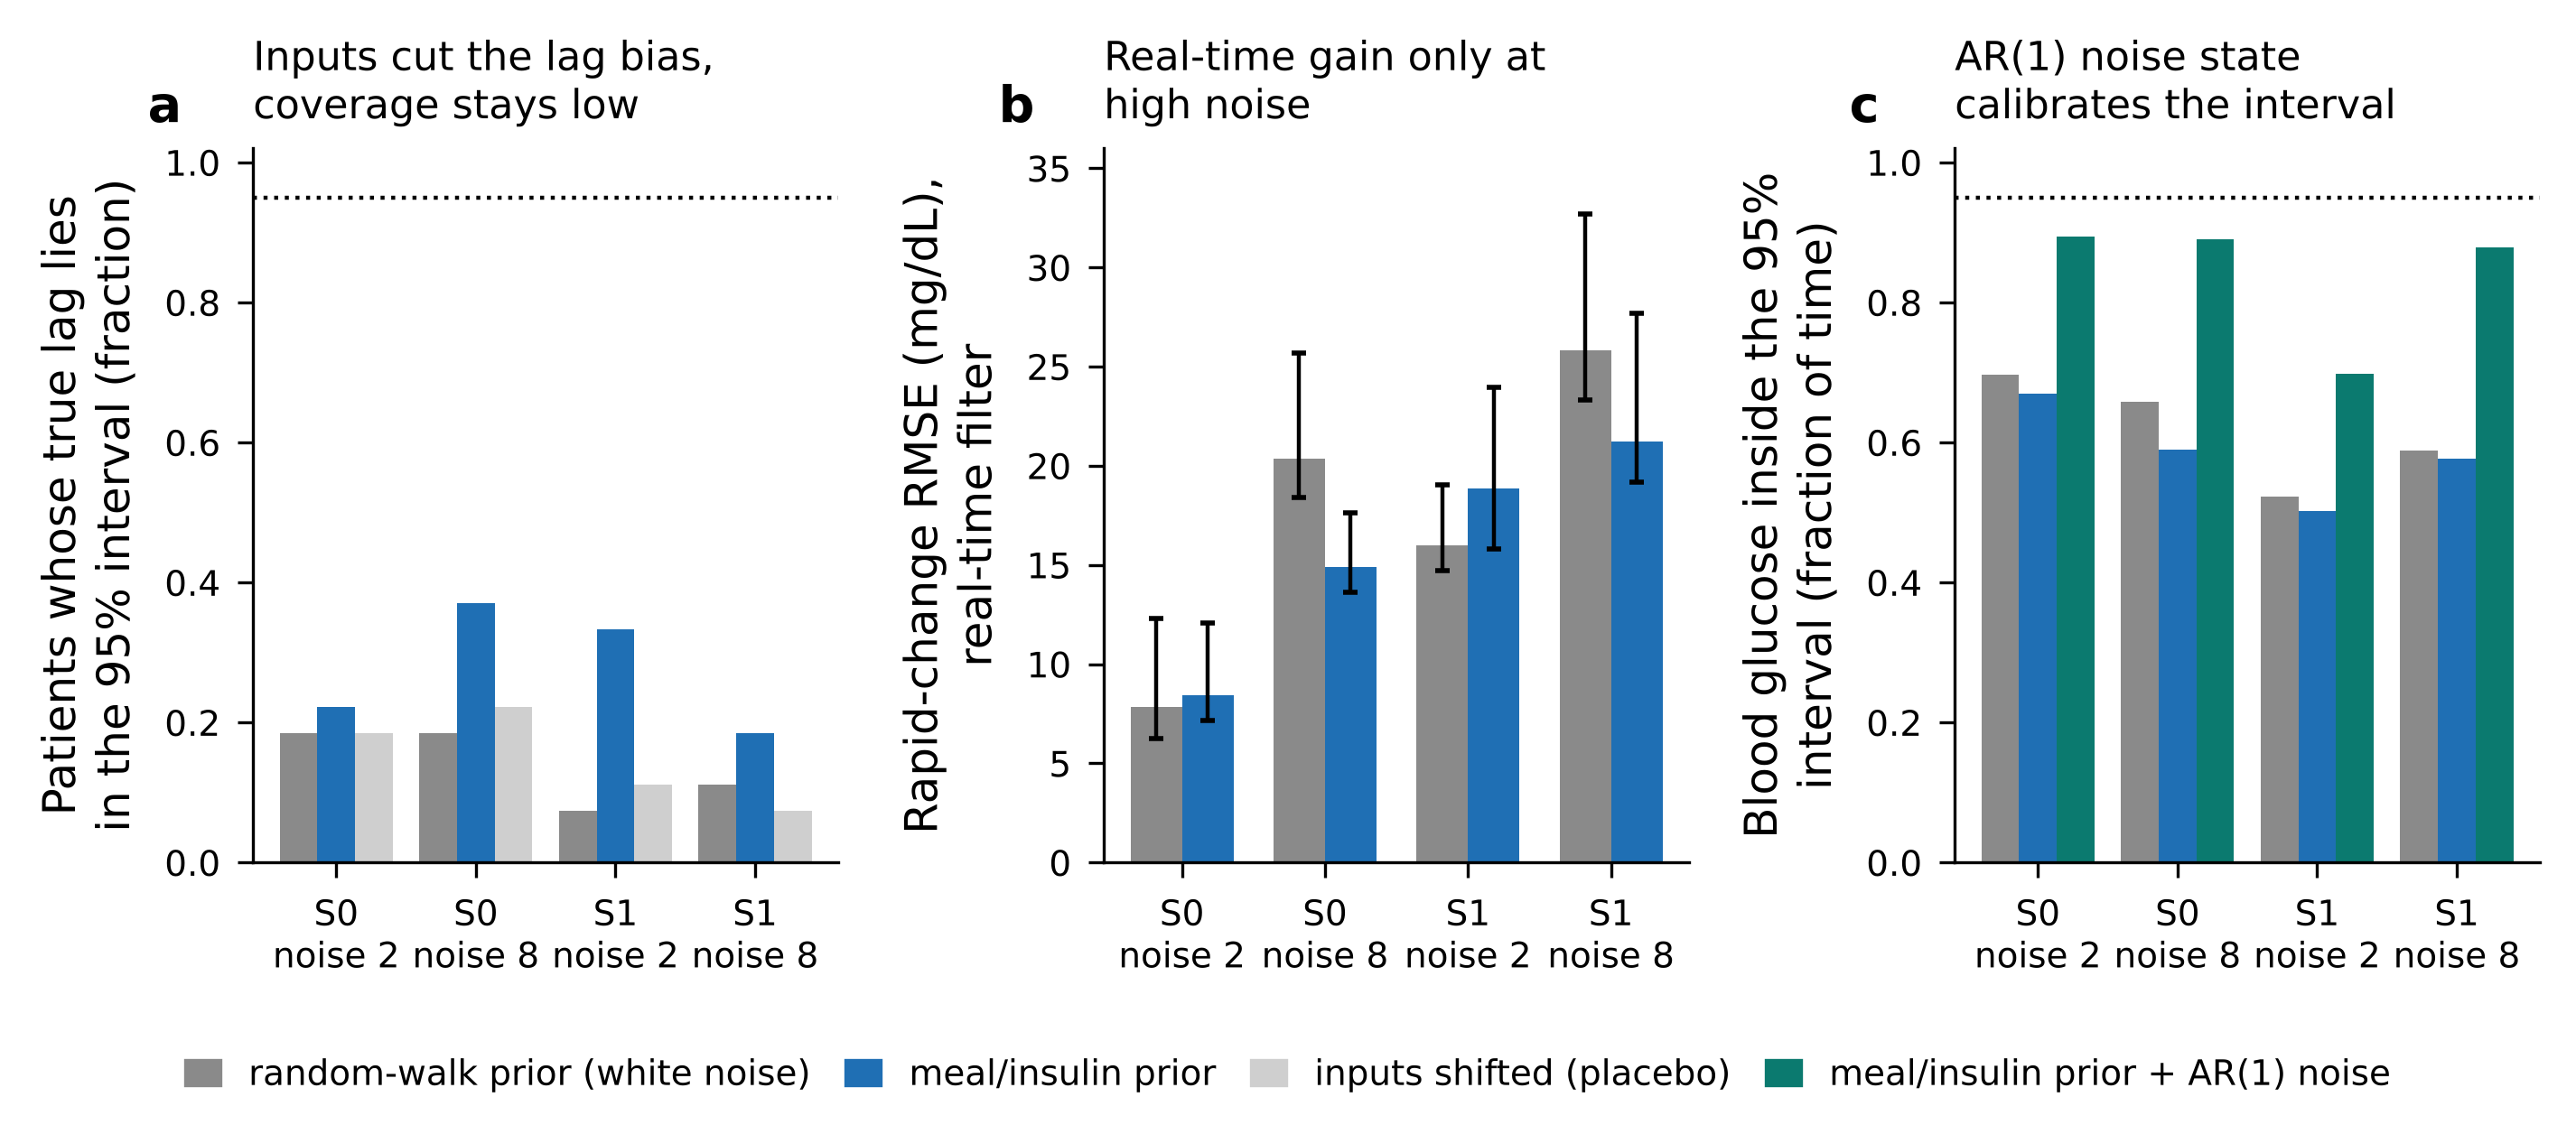
\includegraphics[width=\linewidth]{../../results/fig_pieces678.png}
\caption{Pieces 6 and 8. (a) Fraction of patients whose true effective lag lies in the 95\% likelihood interval. (b) Rapid-change RMSE of the real-time filter, median with bootstrap 95\% CI. (c) Fraction of days 4--5 inside the smoother's 95\% interval, noise settings chosen by likelihood. 27 simulated patients; S0 matched sensor, S1 adds filter and delay; dotted line is the nominal 95\%.}\end{figure}

\section{Real data}
The OhioT1DM loader and a leave-one-patient-out fingerstick check are implemented and tested on synthetic files in the dataset's XML format, but \textbf{have not been run on real data}: the dataset requires a data-use agreement, and a request draft is in the repository. Fingersticks are noisy and sparse and may have been used to calibrate the CGM, so any real-data result is exploratory.

\section{Limitations}
\begin{itemize}
\item Simulation only; the lag is exactly first-order in the simulator, so matched results are best-case.
\item The input prior uses exact logged meals and insulin; real logs are noisy and incomplete, so Piece 6 gains are an upper bound.
\item The AR(1) noise structure used in Piece 8 is the simulator's own (an oracle structure); real sensor noise is unknown.
\item Fingerstick timing and error models, kernel constants and grids are assumptions; tuning grids are coarse.
\item Hypoglycaemia is over-represented in the simulated patients.
\end{itemize}

\section{Conclusion}
Under this simulation, the lag is best handled retrospectively and as a population effective lag calibrated against fingersticks, not as a per-patient parameter identified from CGM alone. Meal and insulin logs improve the state estimate and an AR(1) noise state calibrates the uncertainty, but neither makes individual lag identifiable. The next test is real data with fingerstick references.

\begin{thebibliography}{9}
\bibitem{basu2013} A. Basu \emph{et al.}, ``Time lag of glucose from intravascular to interstitial compartment in humans,'' \emph{Diabetes}, vol.~62, no.~12, pp.~4083--4087, 2013. doi:10.2337/db13-1132
\bibitem{schmelzeisen2015} G. Schmelzeisen-Redeker \emph{et al.}, ``Time delay of CGM sensors: relevance, causes, and countermeasures,'' \emph{J. Diabetes Sci. Technol.}, vol.~9, no.~5, pp.~1006--1015, 2015. doi:10.1177/1932296815590154
\bibitem{dallaman2014} C. Dalla Man \emph{et al.}, ``The UVA/PADOVA type 1 diabetes simulator: New features,'' \emph{J. Diabetes Sci. Technol.}, vol.~8, no.~1, pp.~26--34, 2014. doi:10.1177/1932296813514502
\end{thebibliography}
\end{document}
